\documentclass{beamer}

\usepackage[utf8]{inputenc}
\usepackage{fancybox,fancyvrb}
\usepackage{environ}
\usepackage{tikz}

\beamertemplatenavigationsymbolsempty
\setbeamertemplate{footline}[frame number]
\usetheme{Pittsburgh}

\newcommand{\grad}{\nabla}
\newcommand{\ih}{\boldsymbol{\hat{\textbf{\i}}}}
\newcommand{\jh}{\boldsymbol{\hat{\textbf{\j}}}}
\newcommand{\vF}{\boldsymbol{\vec{\textbf{F}}}}

\title{2.4 Exact (first-order differential) Equations}

\subtitle{a lesson for MATH F302 Differential Equations}

\author{Ed Bueler, Dept.~of Mathematics and Statistics, UAF}

\date{\tiny \today}


\begin{document}
\setbeamertemplate{itemize item}{$\bullet$}
\setbeamertemplate{itemize subitem}{$\circ$}

\begin{frame}
\titlepage

\centerline{\tiny for textbook: \, D. Zill, \emph{A First Course in Differential Equations with Modeling Applications}, 11th ed.}
%\color{green!40!blue}
\end{frame}


\begin{frame}{three objects from calculus III}

to get started on exact equations we recall these two ideas:
\begin{enumerate}
\item \begin{minipage}[t]{0.4\textwidth}
\emph{vector fields}:
    $$\vF = a(x,y) \ih + b(x,y) \jh$$

\vspace{-3mm}
    \begin{itemize}
    \small
    \item like a slope field

    \vspace{-2mm}
    \item \dots but with magnitudes
    \end{itemize}
\end{minipage}
\begin{minipage}[t]{0.5\textwidth}
\vspace{-2mm}

\hfill 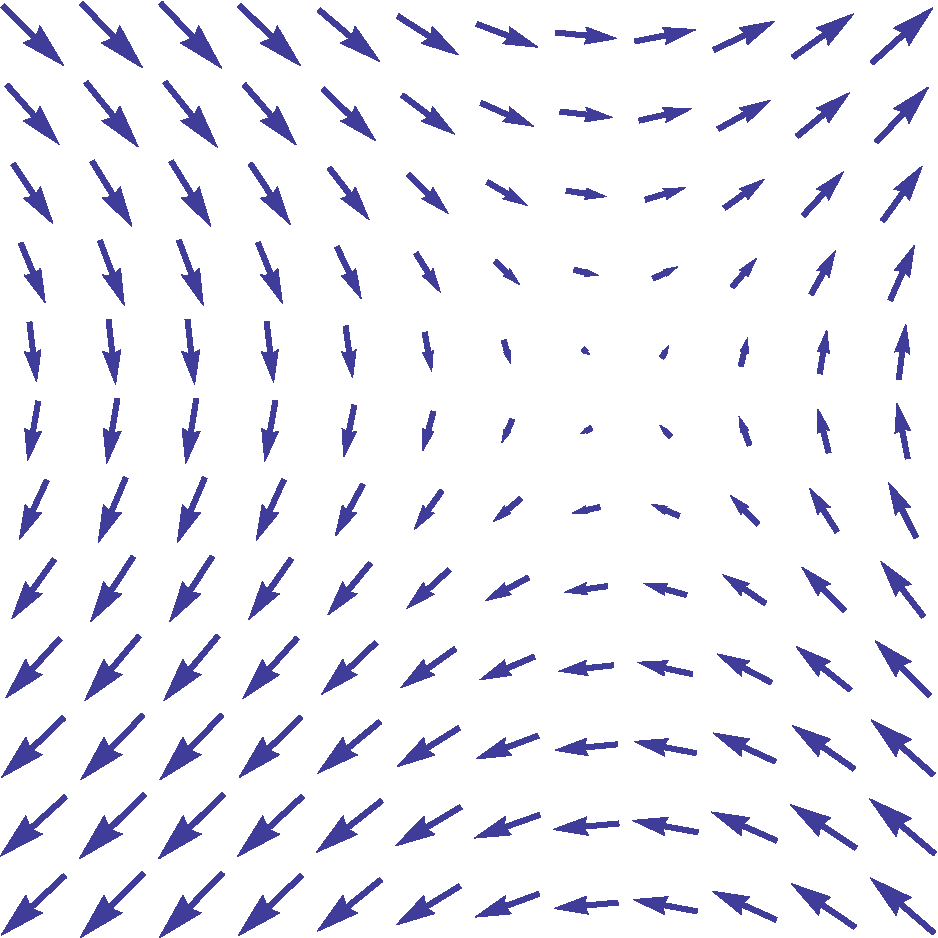
\includegraphics[width=0.5\textwidth]{figs/VectorField}

\hfill \tiny $\boldsymbol{\vec{\textbf{F}}} = \sin y \ih + \sin x \jh$
\end{minipage}

\vspace{-3mm}
\item the \emph{gradient} of a function $f(x,y)$:
    $$\grad f(x,y) = \frac{\partial f}{\partial x} \ih + \frac{\partial f}{\partial y} \jh$$

    \vspace{-2mm}
    \begin{itemize}
    \item the gradient \emph{is} a vector field:  $a=\frac{\partial f}{\partial x}$, $b=\frac{\partial f}{\partial y}$
    \item the gradient points uphill on the surface $z=f(x,y)$
    \end{itemize}
\item the \emph{differential} of $f$ contains the same information as the gradient: $df = \frac{\partial f}{\partial x}\,dx + \frac{\partial f}{\partial y}\,dy$
\end{enumerate}
\end{frame}


\begin{frame}{a major idea}

\begin{itemize}
\item \emph{not obvious but true}: some vector fields are gradients and some are not!

\medskip
    \begin{itemize}
    \item Example: $\vF=\cos(x+y)\ih + (y+\cos(x+y))\jh$ \emph{is} a gradient
        $$\text{supply an $f$:} \hspace{4.0in}$$
        % f(x,y) = \frac{1}{2} y^2 + \sin(x+y)

\medskip
    \item Example: $\vF=\cos(x+y)\ih + (x+\cos(x+y))\jh$ is \emph{not} a gradient
        $$\text{explain why: \hspace{1.0in} \dots ?} \hspace{2.0in}$$
        % dM/dy = -\sin(x+y),  dN/dx = 1 - \sin(x+y)
    \end{itemize}
\item \emph{same idea}: some forms
    $$M(x,y)\,dx + N(x,y)\,dy$$
are the differentials of an $f$---they're \alert{exact}---and some are not
\end{itemize}
\end{frame}


\begin{frame}{recall differentials}

\begin{itemize}
\item \emph{differentials} were introduced in calc.~I as a way to think about linearizations: $df = f'(x)\,dx$
\item for ODEs we need differentials for functions of 2 variables:
    $$f=f(x,y) \qquad \implies \qquad df = \frac{\partial f}{\partial x}\,dx + \frac{\partial f}{\partial y}\,dy$$

\vspace{-2mm}
    \begin{itemize}
    \item differential of $f(x,y)$ describes the tangent plane to the surface $z=f(x,y)$
    \item the differential contains the same information as the gradient
    \item \alert{note:} you need to be able to compute partial derivatives!
    \end{itemize}
\item Example: find the differential of $f(x,y)=\frac{1}{2} y^2 + \sin(x+y)$

\vspace{20mm}
\end{itemize}
\end{frame}


\begin{frame}{how this relates to DEs}

\begin{itemize}
\item \emph{definition:}  a differential form
    $$M(x,y)\,dx + N(x,y)\,dy$$
is \emph{exact} if there is $f(x,y)$ so that the form is a differential:
    $$M = \frac{\partial f}{\partial x}, \qquad N = \frac{\partial f}{\partial y}$$
\item \alert{main idea:} if we can rewrite an ODE as an exact differential form then we can solve the ODE
\end{itemize}
\end{frame}


\begin{frame}{example 1}

\begin{columns}
\begin{column}{0.6\textwidth}
\begin{itemize}
\item I will do an example
\item \dots uses ``miracle'' at one step
\item \dots not sustainable
\item Example 1: solve
    $$y' = \frac{2y}{3y-2x}$$

\vspace{30mm}
\end{itemize}
\end{column}
\begin{column}{0.4\textwidth}
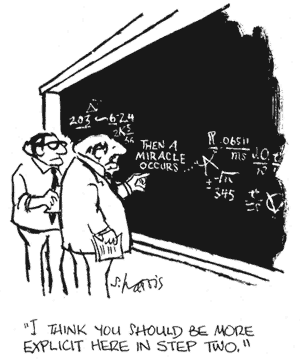
\includegraphics[width=\textwidth]{figs/miracle}

\vspace{20mm}
\end{column}
\end{columns}
\end{frame}

\begin{frame}{example 1, cont.}

\begin{itemize}
\item Example 1: solve
    $$y' = $$
\end{itemize}
\end{frame}

\begin{frame}{X}

\begin{itemize}
\item X
\item 
\end{itemize}
\end{frame}

\begin{frame}{X}

\begin{itemize}
\item X
\item 
\end{itemize}
\end{frame}

\begin{frame}{expectations}

to learn this material, just watching this video is \emph{not} enough; also
\begin{itemize}
\item \emph{watch} ``found online'' videos at

\centerline{\href{https://bueler.github.io/math302/week4.html}{\tt \color{cyan} bueler.github.io/math302/week4.html}}
\item \emph{try-out} Euler's method codes at the same link
\item \emph{read} section 2.4 in the textbook
\item \emph{do} the WebAssign exercises for section 2.4
\end{itemize}
\end{frame}

\end{document}

